\documentclass[12pt]{article}
\usepackage{graphicx}
\usepackage{geometry}
\usepackage{pdfpages}
\usepackage{titlesec}
\usepackage{centernot}
\usepackage{fancyhdr}
\usepackage{hyperref}
\usepackage{float}     % For [H] placement option in figures
% Margins
\geometry{
    a4paper,
    total={170mm,257mm},
    left=20mm,
    top=20mm,
}

\begin{document}

% Title page
\begin{titlepage}
    \centering
    \vspace*{5cm}
    
    {\Huge \textbf{MEC6602E: Transonic Aerodynamics}}\\[1.5cm]
    
    {\Large \textbf{HOMEWORK 2}}\\[2cm]
    
    {\Large Prepared by:}\\
    {\Large Kamal Jemmali 2019339}\\
    {\Large Hugo Javourez 2420717}\\[1.5cm]
    
    {\Large Submitted to :}\\
    {\Large M.Frédéric Plante. Ph.D, CPI}\\[2cm]
    
    {\Large Due date :}\\
    {\Large 28 Octobre 2024}\\
    
    \vfill
    
\includegraphics[width=0.25\textwidth]{polytechnique-signature-rgb-gauche-fr.png} % Placeholder for a logo or image (optional)
    
    \vfill
\end{titlepage}

The main goal is to simulate a shock tube, 2 nozzles case, the first one is the supersonic input and output,
and the second one is the supersonic input and subsonic output. In this report, we will show the density, rho, and mack number over x.
.Futhermore, we will show error L2 in fonction of the numbers of iterations. We will also do the simulation at differents CFL.
Please refer is 

\section{Macmormack Simulations}

Before any analysis, We will show the results we got at differents parameters. 

\subsection{Shock Tube}

\subsubsection{results}

\begin{figure}[H] % Use [p] to place the figure on a separate page
    \centering
    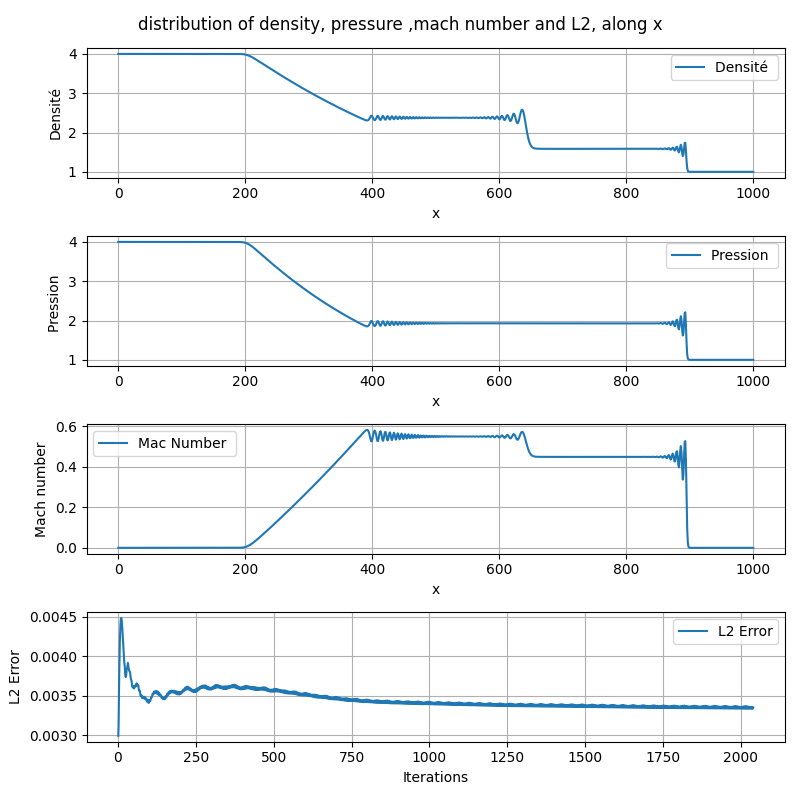
\includegraphics[width=\textwidth,height=\textheight,keepaspectratio]{PLOTS/tube_macormack_CFL25.png}
    \caption{Tube Maccormack simulation at CFL 0.25}
    \label{fig:your_label}
\end{figure}

\begin{figure}[H] % Use [p] to place the figure on a separate page
    \centering
    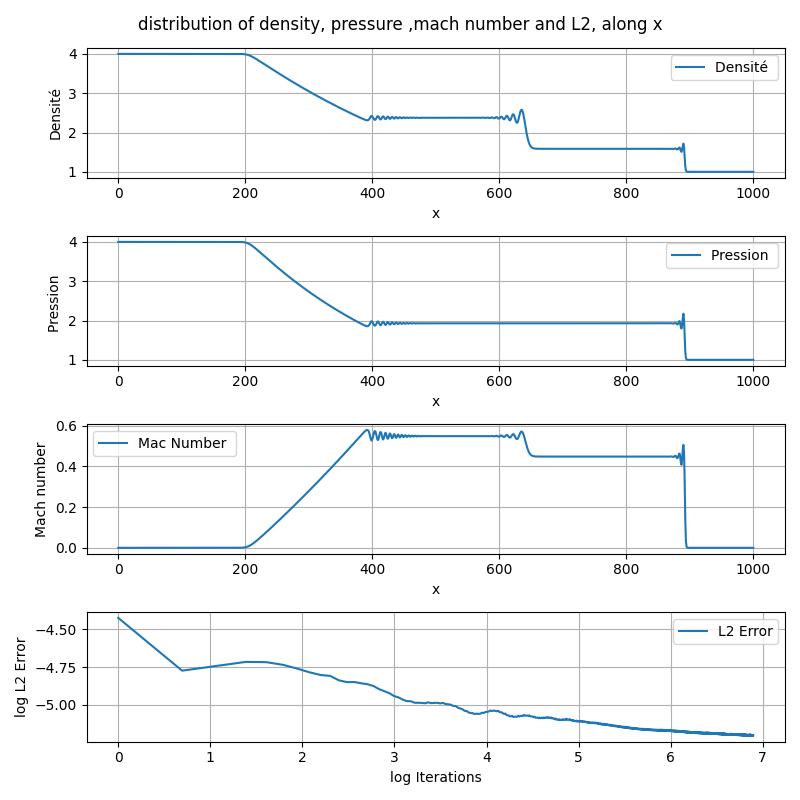
\includegraphics[width=\textwidth,height=\textheight,keepaspectratio]{PLOTS/tube_macormack_CFL05.png}
    \caption{Tube Maccormack simulation at CFL 0.50}
    \label{fig:your_label}
\end{figure}

\begin{figure}[H] % Use [p] to place the figure on a separate page
    \centering
    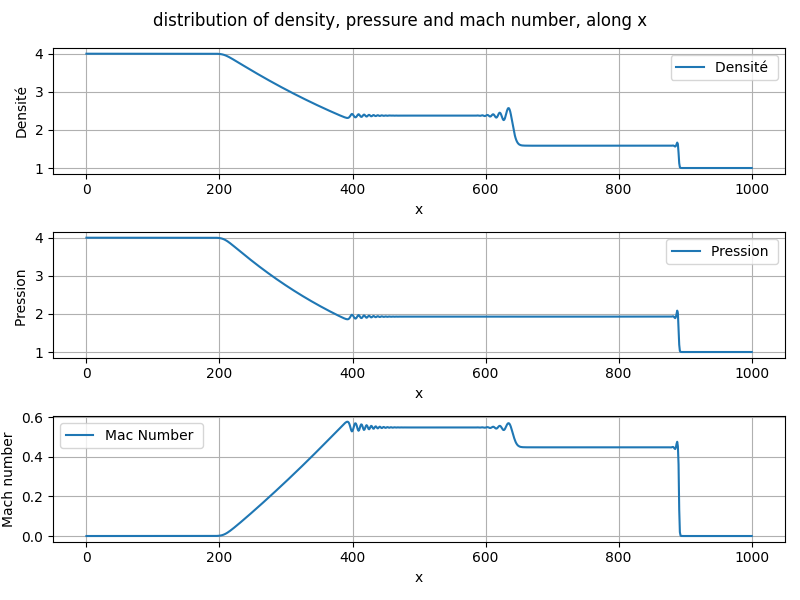
\includegraphics[width=\textwidth,height=\textheight,keepaspectratio]{PLOTS/tube_macormack_CFL75.png}
    \caption{Tube Maccormack simulation at CFL 0.75}
    \label{fig:your_label}
\end{figure}

\begin{figure}[H] % Use [p] to place the figure on a separate page
    \centering
    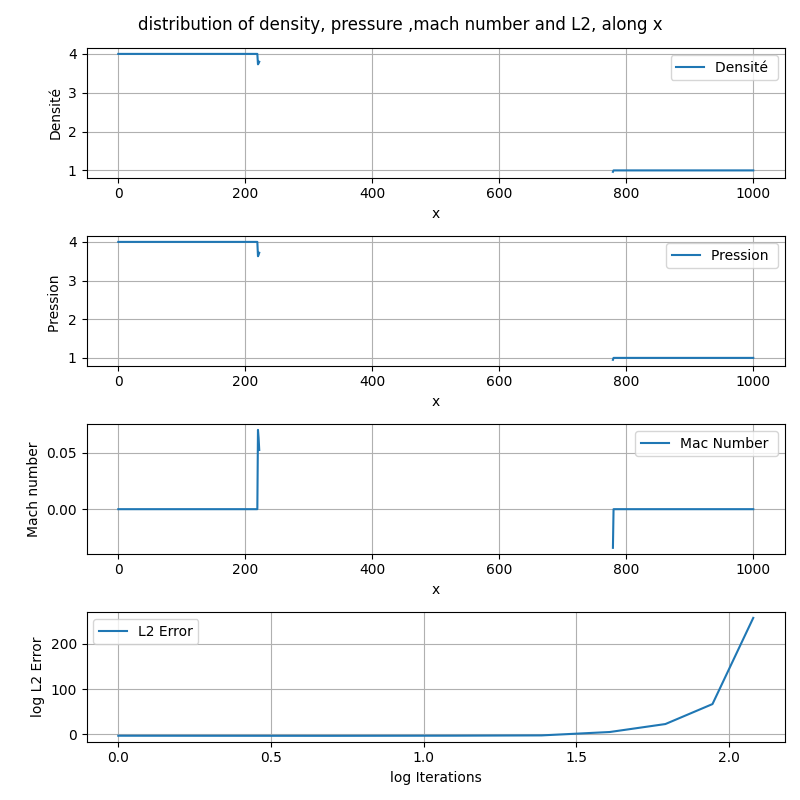
\includegraphics[width=\textwidth,height=\textheight,keepaspectratio]{PLOTS/tube_macormack_CFL110.png}
    \caption{Tube Maccormack simulation at CFL 1.1}
    \label{fig:your_label}
\end{figure}

\subsubsection{Analysis}

As we can see, for $ 0 < CFL < 1$, The scheme converge to a certain solutions that is the solution given is the .dat file
.We can also see that the scheme is stable because the L2 gets lowers when there is more iterations. As exepected, thios does 
not happen when the $CFL > 1$ Because this is an explicit scheme

\subsection{SuperSonic - Supersonic Nozzle}

\subsubsection{results}
\begin{figure}[H] % Use [p] to place the figure on a separate page
    \centering
    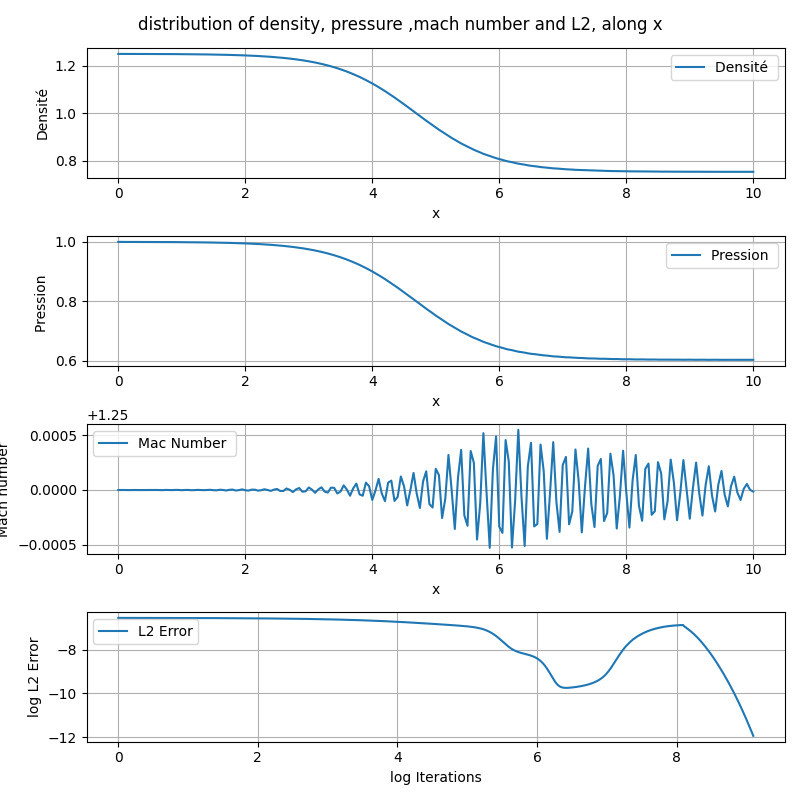
\includegraphics[width=\textwidth,height=\textheight,keepaspectratio]{PLOTS/Tuyere_super_super_Macormack_CFL050.png}
    \caption{Tuyère supersonic-supersonic at CFL = 0.5}
    \label{fig:your_label}
\end{figure}
\begin{figure}[H] % Use [p] to place the figure on a separate page
    \centering
    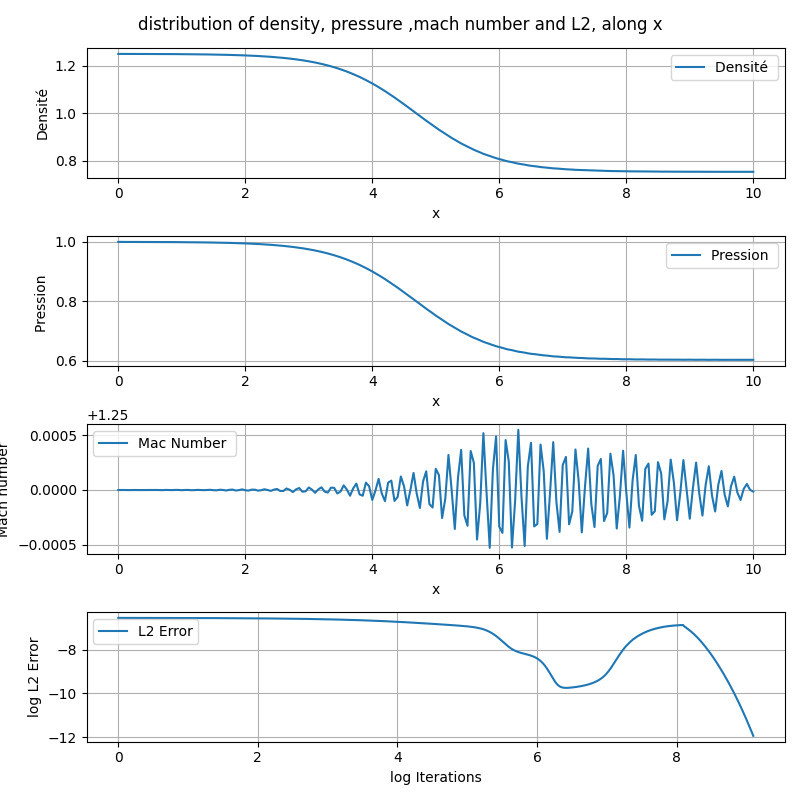
\includegraphics[width=\textwidth,height=\textheight,keepaspectratio]{PLOTS/Tuyere_super_super_Macormack_CFL050.png}
    \caption{Tuyère supersonic-supersonic at CFL = 0.5}
    \label{fig:your_label}
\end{figure}
\begin{figure}[H] % Use [p] to place the figure on a separate page
    \centering
    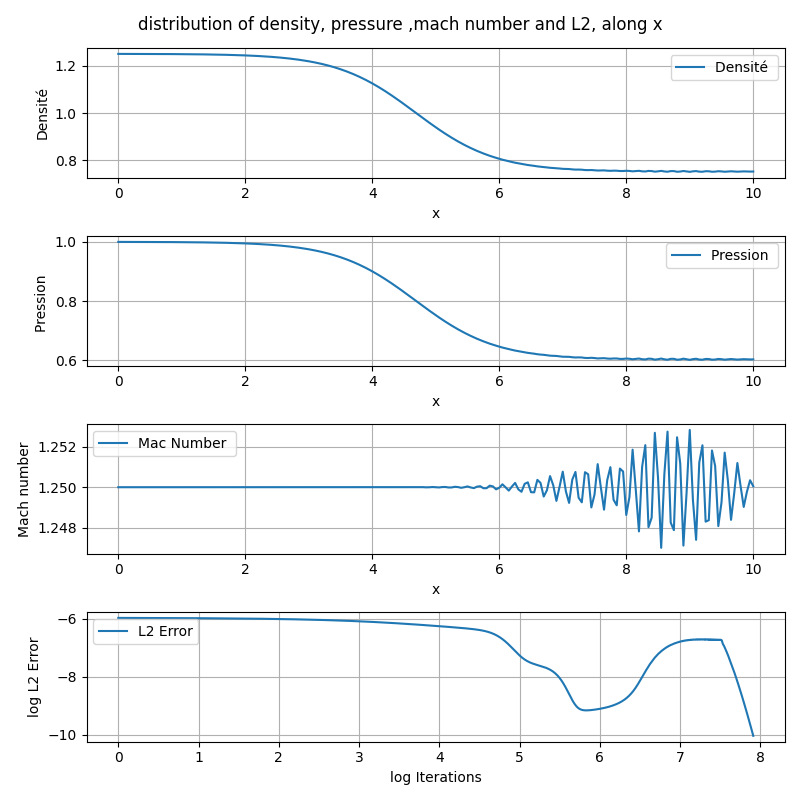
\includegraphics[width=\textwidth,height=\textheight,keepaspectratio]{PLOTS/Tuyere_super_super_Macormack_CFL090.png}
    \caption{Tuyère supersonic-supersonic at CFL = 0.90}
    \label{fig:your_label}
\end{figure}

\begin{figure}[H] % Use [p] to place the figure on a separate page
    \centering
    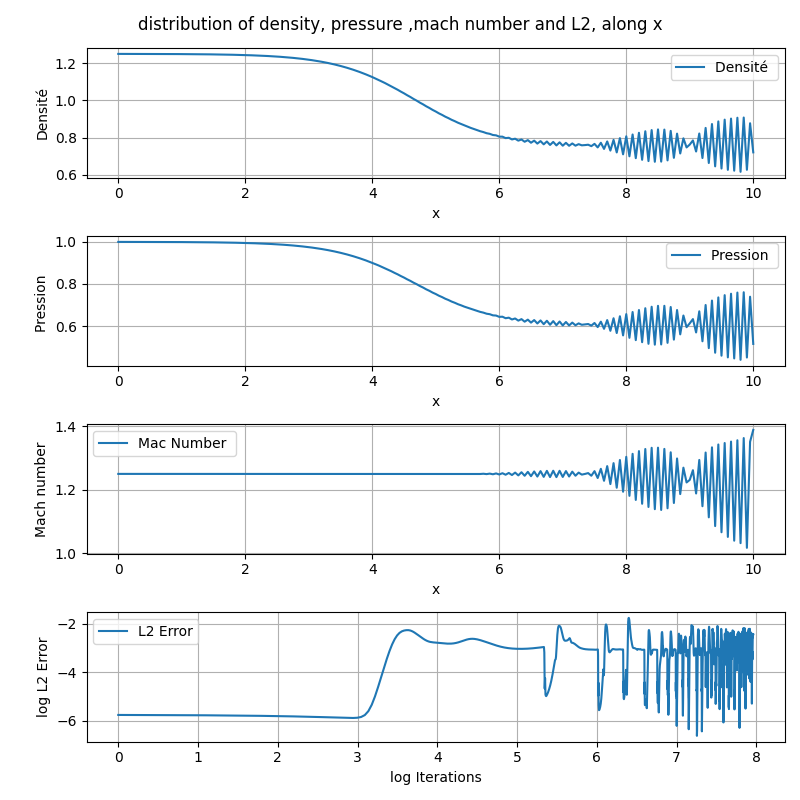
\includegraphics[width=\textwidth,height=\textheight,keepaspectratio]{PLOTS/Tuyere_super_super_Macormack_CFL110.png}
    \caption{Tuyère supersonic-supersonic at CFL = 1.10}
    \label{fig:your_label}
\end{figure}

\subsubsection{Analysis}
This is what we were expection, a drop in density and pressure when it stabilise and the mach number becoming 1.25 everywhere. 
Careful, the mach number seems to be instable at the outlet, but please pay attention to the y-axis, you will see that its quite stable. 
As expected, the CFL number has an influence here. Its should not be higher than 1. 


\subsection{SuperSonic - Subsonic Nozzle}
\subsubsection{results}
\begin{figure}[H] % Use [p] to place the figure on a separate page
    \centering
    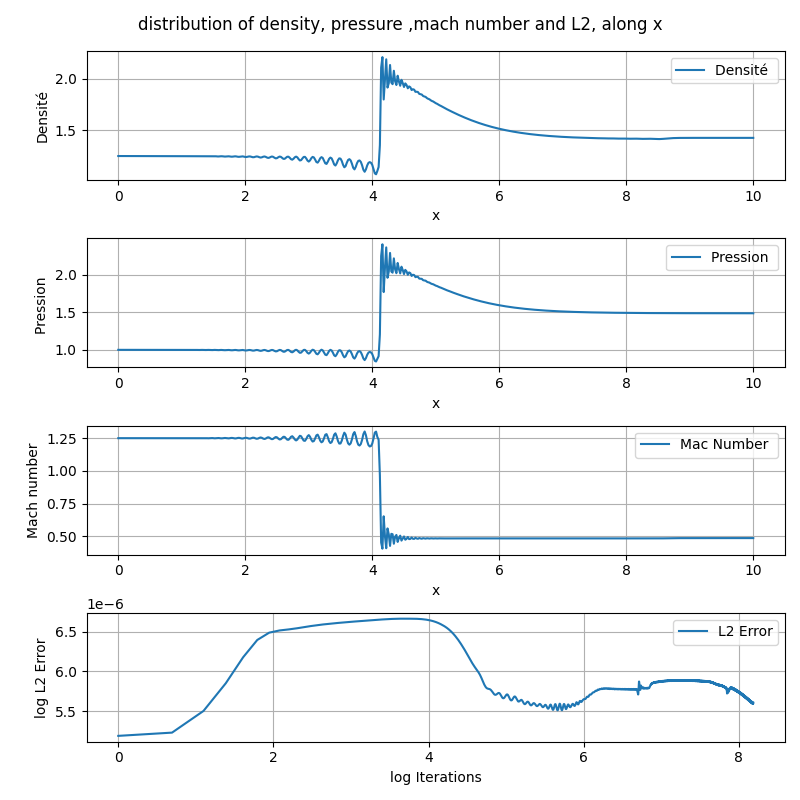
\includegraphics[width=\textwidth,height=\textheight,keepaspectratio]{PLOTS/Tuyere_super_sub_Macormack_CFL06.png}
    \caption{Tuyère supersonic-subsonic at CFL = 0.6}
    \label{fig:your_label}
\end{figure}

\begin{figure}[H] % Use [p] to place the figure on a separate page
    \centering
    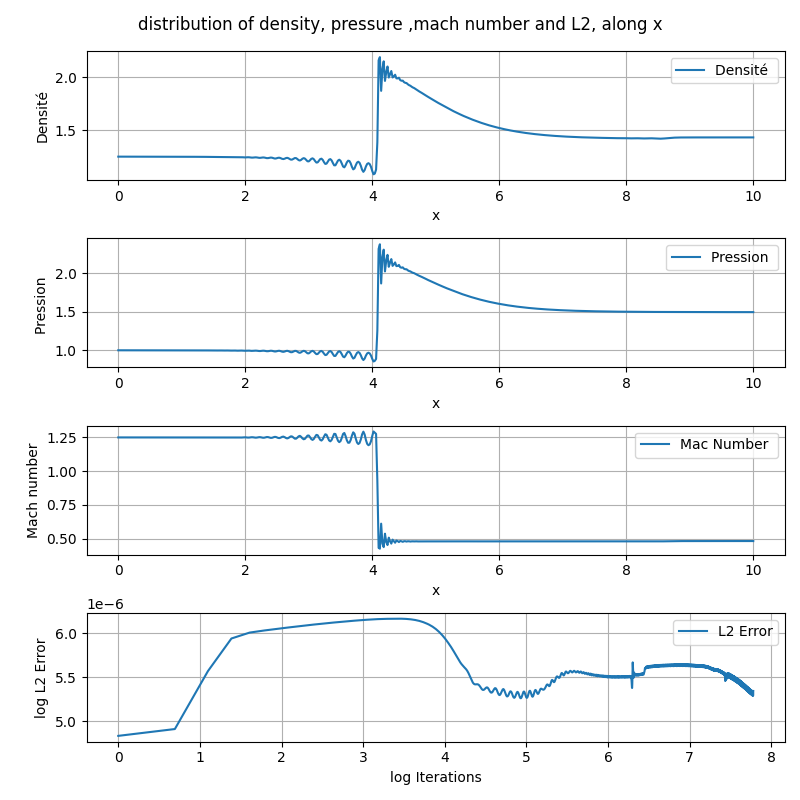
\includegraphics[width=\textwidth,height=\textheight,keepaspectratio]{PLOTS/Tuyere_super_sub_Macormack_CFL09.png}
    \caption{Tuyère supersonic-subsonic at CFL = 0.9}
    \label{fig:your_label}
\end{figure}

\begin{figure}[H] % Use [p] to place the figure on a separate page
    \centering
    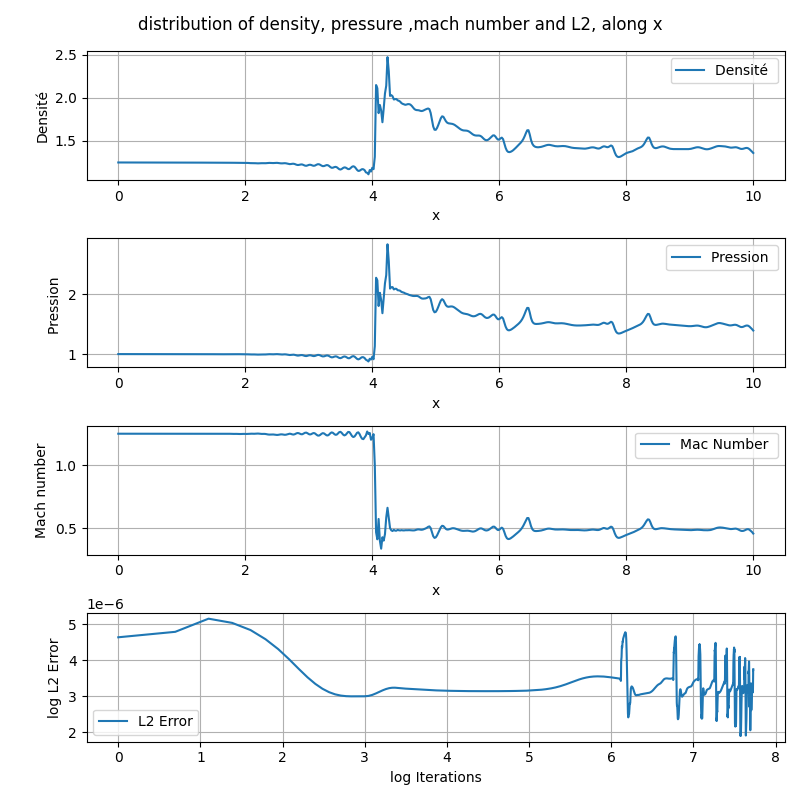
\includegraphics[width=\textwidth,height=\textheight,keepaspectratio]{PLOTS/Tuyere_super_sub_Macormack_CFL11.png}
    \caption{Tuyère supersonic-subsonic at CFL = 1.1}
    \label{fig:your_label}
\end{figure}
\subsubsection{analysis}
As we can see here, those result are the same results given at the manual, we were expecting a big drop on speed, while the pressure and density explode at the end
which is something quite logical. Here, When the $cfl>1$ we get something quite right with alot of instability, but it never diverges. 
\section{ANNEXE 2: GITHUB LINK}

\href{https://github.com/Kenesis69/MEC_6602E_HOMEWORK_2}{Click for Github Acces}

\end{document}
